Um espaço de cores é um modelo matemático utilizado para descrever uma determinada cor representando um \emph{gamut}, uma paleta de cores que uma certa tecnologia é capaz de reproduzir. Existem diversos modelos de espaços de cores, tais como RGB e CIELab, os quais possuem diferentes  formas de representação \cite{ref:galleti}.

A sigla RGB é uma abreviatura de um espaço de cores formado por três canais: um R, que vem do inglês \emph{red} (vermelho); outro G, do inglês \emph{green} (verde); e o outro B, do inglês \emph{blue} (azul). O RGB forma a síntese aditiva em que, pela sobreposição das três luzes em um ambiente totalmente escuro, obtém-se a luz branca, como ilustrado na Figura \ref{fig:rgb}. Em cada um dos três canais deste espaço de cores, um valor de intensidade é atribuído para cada \emph{pixel} de uma imagem, variando de $0$ a $255$. Essa atribuição tem como finalidade a composição de uma imagem colorida e é muito utilizada na indústria gráfica digital e em mídias digitais, como televisão, câmeras, escâneres, \emph{smartphones}, etc \cite{ref:galleti}.

\begin{figure}[h]
	\centering
	\caption{Síntese aditiva do espaço de cores RGB. Fonte: \cite{ref:galleti}.}
	\label{fig:rgb}
	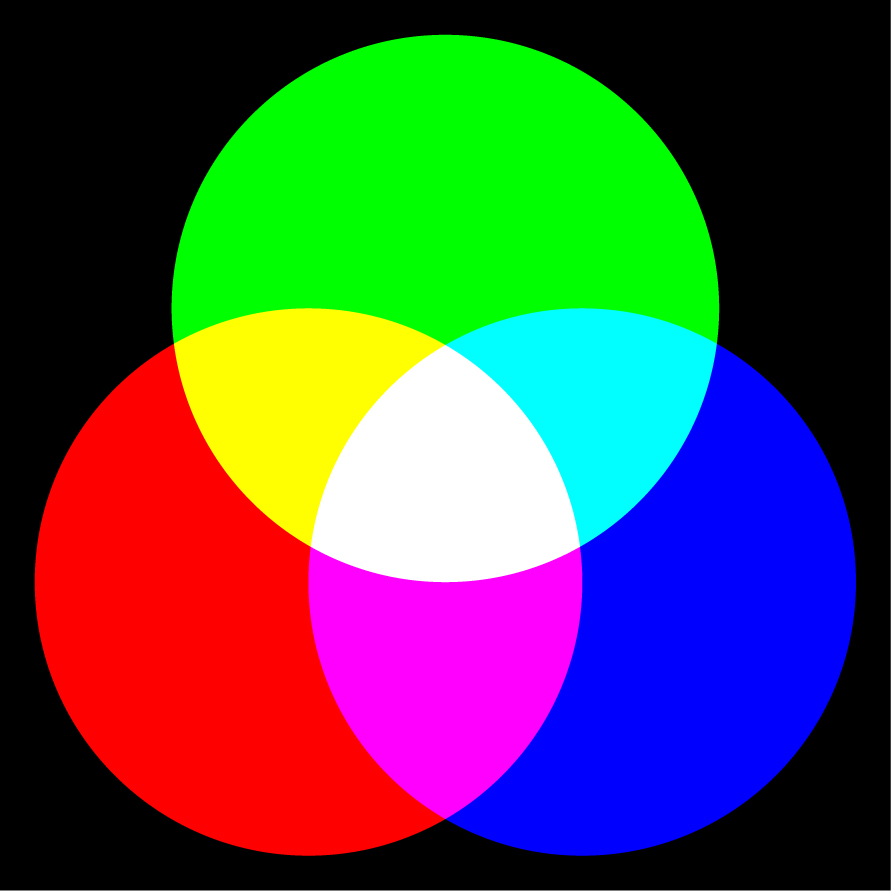
\includegraphics[width=0.3\textwidth]{./img/rgb}
\end{figure}


A \emph{Commision Internationale L'Eclairage} (CIE), deu nome a um outro espaço de cores bastante utilizado como referência para gerenciamento de cores no tratamento de imagens, o CIELab. A sigla Lab retrata os três canais utilizados por esse sistema os quais estão graficamente representados na Figura \ref{fig:cielab}. O canal simbolizado pela letra $L$ indica luminosidade, variando de preto a branco e os canais das letras $a$ e $b$ são os eixos de cromaticidade, em que $a$ varia de vermelho a verde e $b$ varia de azul a amarelo. Nesse modelo, a separação de cores é feita de maneira a deixar um canal responsável pela formação do desenho da imagem (canal $L$), e os outros dois canais ($a$ e $b$) ficam responsáveis apenas pelas informações das cores \cite{ref:galleti}.

\begin{figure}[h]
	\centering
	\caption{Representação gráfica do espaço de cores CIELab. Fonte: \cite{ref:galleti}.}
	\label{fig:cielab}
	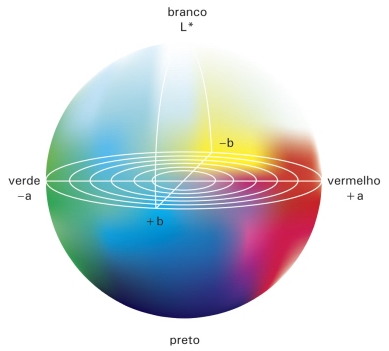
\includegraphics[width=0.5\textwidth]{./img/cielab}
\end{figure}

